% THIS IS SIGPROC-SP.TEX - VERSION 3.1
% WORKS WITH V3.2SP OF ACM_PROC_ARTICLE-SP.CLS
% APRIL 2009
%
% It is an example file showing how to use the 'acm_proc_article-sp.cls' V3.2SP
% LaTeX2e document class file for Conference Proceedings submissions.
% ----------------------------------------------------------------------------------------------------------------
% This .tex file (and associated .cls V3.2SP) *DOES NOT* produce:
%       1) The Permission Statement
%       2) The Conference (location) Info information
%       3) The Copyright Line with ACM data
%       4) Page numbering
% ---------------------------------------------------------------------------------------------------------------
% It is an example which *does* use the .bib file (from which the .bbl file
% is produced).
% REMEMBER HOWEVER: After having produced the .bbl file,
% and prior to final submission,
% you need to 'insert'  your .bbl file into your source .tex file so as to provide
% ONE 'self-contained' source file.
%
% Questions regarding SIGS should be sent to
% Adrienne Griscti ---> griscti@acm.org
%
% Questions/suggestions regarding the guidelines, .tex and .cls files, etc. to
% Gerald Murray ---> murray@hq.acm.org
%
% For tracking purposes - this is V3.1SP - APRIL 2009

\documentclass{acm_proc_article-sp}

\begin{document}

\title{Benchmarking In-Memory Streaming Database Management Systems}
\subtitle{[Extended Abstract]}
%
% You need the command \numberofauthors to handle the 'placement
% and alignment' of the authors beneath the title.
%
% For aesthetic reasons, we recommend 'three authors at a time'
% i.e. three 'name/affiliation blocks' be placed beneath the title.
%
% NOTE: You are NOT restricted in how many 'rows' of
% "name/affiliations" may appear. We just ask that you restrict
% the number of 'columns' to three.
%
% Because of the available 'opening page real-estate'
% we ask you to refrain from putting more than six authors
% (two rows with three columns) beneath the article title.
% More than six makes the first-page appear very cluttered indeed.
%
% Use the \alignauthor commands to handle the names
% and affiliations for an 'aesthetic maximum' of six authors.
% Add names, affiliations, addresses for
% the seventh etc. author(s) as the argument for the
% \additionalauthors command.
% These 'additional authors' will be output/set for you
% without further effort on your part as the last section in
% the body of your article BEFORE References or any Appendices.

\numberofauthors{2} %  in this sample file, there are a *total*
% of EIGHT authors. SIX appear on the 'first-page' (for formatting
% reasons) and the remaining two appear in the \additionalauthors section.
%
\author{
% You can go ahead and credit any number of authors here,
% e.g. one 'row of three' or two rows (consisting of one row of three
% and a second row of one, two or three).
%
% The command \alignauthor (no curly braces needed) should
% precede each author name, affiliation/snail-mail address and
% e-mail address. Additionally, tag each line of
% affiliation/address with \affaddr, and tag the
% e-mail address with \email.
%
% 1st. author
\alignauthor
John Meehan \\
john@cs.brown.edu
\alignauthor
Jeff Rasley \\
jeffra@cs.brown.edu
}
% Just remember to make sure that the TOTAL number of authors
% is the number that will appear on the first page PLUS the
% number that will appear in the \additionalauthors section.

\maketitle
\begin{abstract}
This is our abstract, where we talk about stuff.
\end{abstract}

% A category with the (minimum) three required fields
\category{H.2.4}{Database Management}{Streaming, Benchmarking}

\terms{Database Management, Streaming, Benchmarking}

\section{Introduction}
This is the super-awesome intro section that talks about our
whole project yo!

\section{Background}
\subsection{Streaming Overview}
In a traditional database management system, data is imported into a relatively static data structure.  A user is able to run any queries necessary in order to retrieve desired information.  Streaming systems take the opposite approach, percieving the data as consistently changing.  Continuous queries are written into the system in order to perform analytics on this flow of information, particularly on a subsection, or window, of time.

For instance, say that a stock broker wishes to purchase a particular stock when a five-minute moving average crosses a particular threshold.  In this case, the incoming ticker price for this stock is the stream of information, a sliding window of five minutes is placed on this stream, and a continuous query aggregates this data to calculate the average.  A filter operator is placed further downstream of the window in order to trigger further operators if the threshold is met.

\subsection{Modern Streaming Systems}
Due to the nature of real-time processing, it is crucial that all processing take place in memory with minimal requests to disk.  Therefore it is not surprising that distributed, main-memory database systems have become the key players in the streaming database research space.  These systems take advantage of the fact that many streaming applications are highly parallizeable in order to distribute the stream processing across multiple worker machines.  In this paper, we compare the popular distributed system, Spark Streaming, to an established commercial system, which we will call this "System-X."

\subsubsection{Spark Streaming}
Spark Streaming builds on Apache Spark, creating a streaming API on top of the existing main-memory distributed system.  Also known as Discretized Streams, this system takes advantage of Spark's resilient NOTE LOOK UP RDDs in order to store streaming state.~\cite{dstreams}  Time intervals are discretized in order to allow Spark to batch all information within a specific interval, similar to Jennifer Widom's CQL. NOTE SITE CQL  Intermediate states are stored in the system, in order to easily calculate windows and compute aggregates.  Applications for Spark are programmed using Scala syntax, and make heavy use of map reduce operations to parallelize its processing.

\subsubsection{System-X} 
System-X is an established streaming system, built on research which helped to define streaming systems at their inception.  It is primarily designed to be highly user-friendly, providing methods to interface with a large number of applications.  System-X makes use of a graphical programming user interface, but also provides its own "Streaming SQL" language.
\section{Methodology}

\subsection{Strategy}
\label{ssec:strategy}
Streaming systems are typically evaluated by two major metrics:
\begin{itemize}
\item \textbf{Throughput:} We evaluate throughput as the number of tuples that a full system is capable of processing per second.
\item \textbf{Latency:} We consider latency numbers to be the period of time between a tuple's generation and when it is fully processed by the streaming system.  The latency number that a window reports each reporting interval is the current time minus the timestamp of its oldest tuple.
\end{itemize}

\subsection{Tuple Generation}
\label{ssec:tuple-gen-meth}
In both of the benchmarks we use in our comparisons, we consider a tuple to be string of text of a fixed number of words, the first of which indicates the tuple's epoch timestamp in milliseconds.  We then append a second timestamp to the tuple at the end of processing.  We calculate our latency by subtracking our initial timestamp from our final timestamp.  We calculate our throughput by counting the number of tuples with an initial timestamp that are processed within the given window of time.

\subsection{Architecture Philosophy}
\label{ssec:arch-phil}
A typical streaming system receives new tuples of data from an outside source via some external connection.  The system then processes the data, stores information as necessary, and then outputs results as another stream to be displayed or used by other applications.  In this work, we are only interested in evaluating the stream processing portion of this process.

When benchmarking specific workloads, we intended to put as little external strain on the system as possible in order to avoid contaminating our results.  The actual streaming system is hosted on a specific number of machines, with separate machines generating tuples and sending them via the network.  In addition, the output is also sent to yet another machine and written to disk there, again minimizing extra strain on the machines actually performing the workload.

\subsection{Benchmarks}

\begin{figure}[b]
\centering
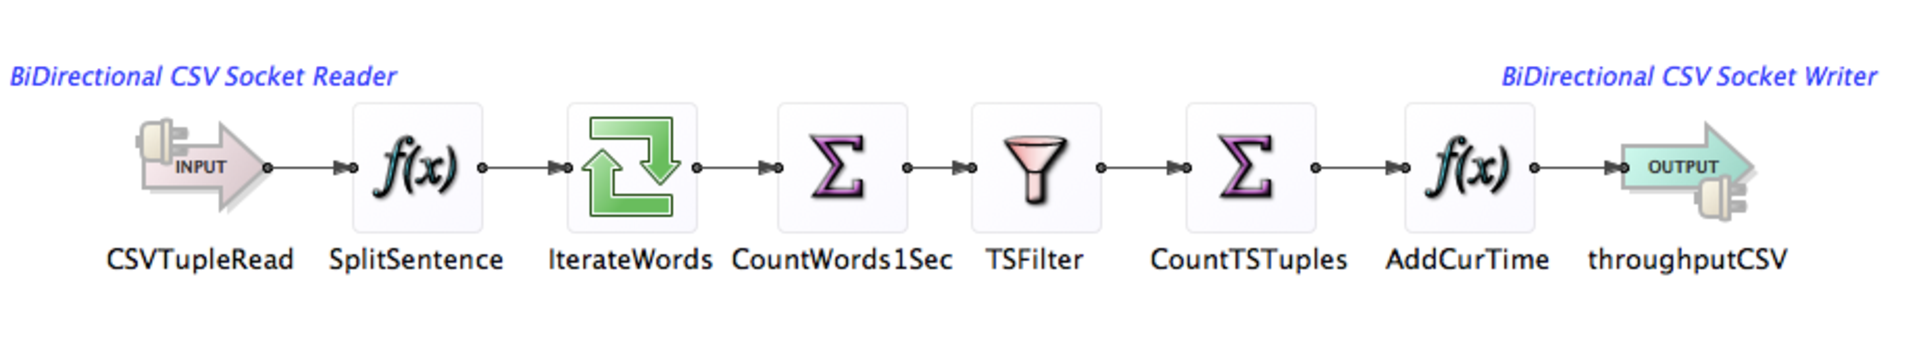
\includegraphics[width=1\linewidth]{figures/System-XWorkflow.pdf}
%\vspace{5.3in}
\caption{Graphical representation of the Wordcount benchmark in System-X}
\label{fig:wordcount}
\end{figure}

We evaluated our systems using two workloads: Wordcount and Grep

\subsubsection{Wordcount}
In the Wordcount benchmark, each input tuple is broken down into individual words and counted within a window of time.  This benchmark should favor Spark, as it is highly parallelizeable.   Spark breaks these tuples into an array of words and then performs map and reduce operations to find their counts.  System-X on the other hand must iterate over each tuple, generate a new tuple for each word, and then perform an aggregation on the resulting tuples.

\subsubsection{Grep}
In the Grep benchmark, input tuples are sent through a filter operation in order to find sentences which contain the word ``the''.  Both Spark and System-X execute similar strategies for this benchmark.

\begin{figure}[t]
\centering
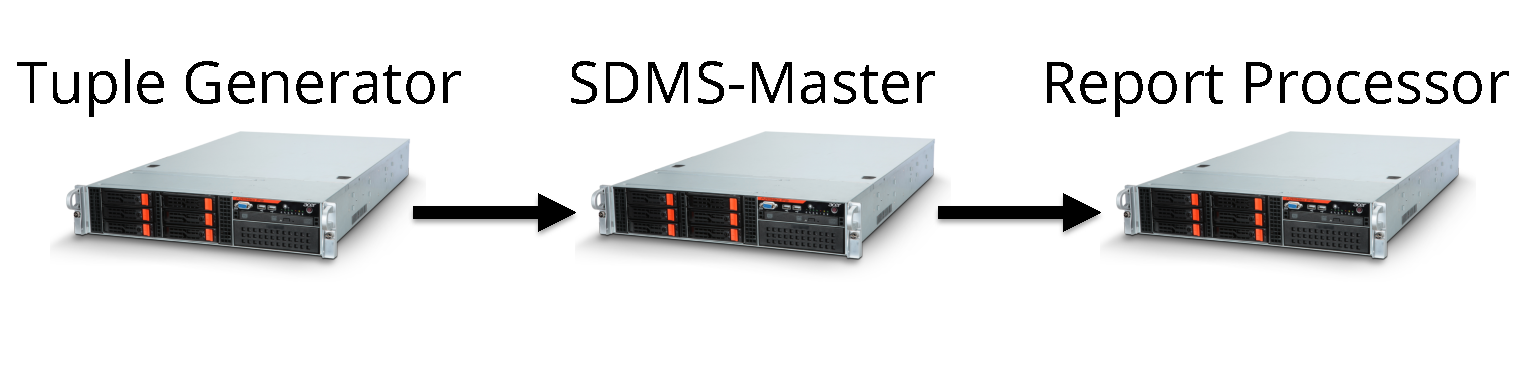
\includegraphics[width=1\linewidth]{figures/diagram.pdf}
%\vspace{-0.3in}
\caption{Single-node cluster setup for benchmarking}
\label{fig:sb1-tput}
\end{figure}

\begin{figure}[b]
\centering
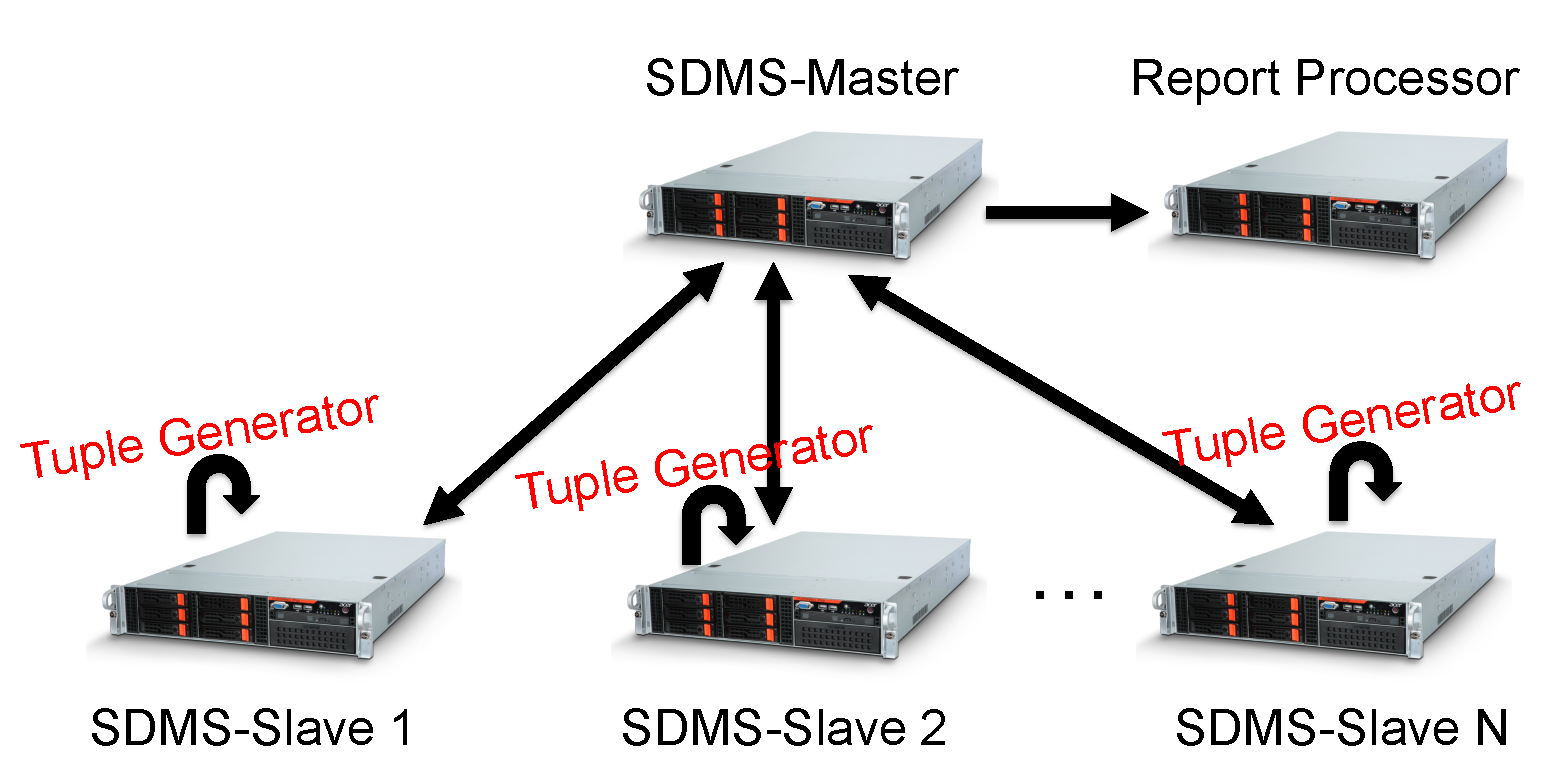
\includegraphics[width=1\linewidth]{figures/spark-full-diagram.pdf}
%\vspace{-0.3in}
\caption{Multi-node cluster setup for benchmarking Spark}
\label{fig:sb1-tput}
\end{figure}




\section{Challenges}
These are our challenges..

\section{Results}
Results!

\begin{figure}[t]
\centering
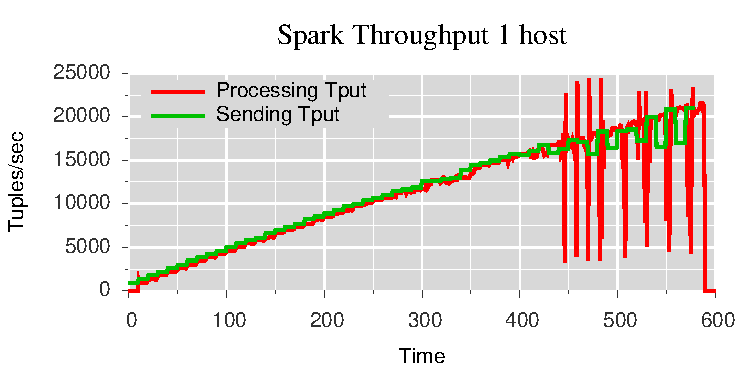
\includegraphics[width=1\linewidth]{figures/sp1_tput.pdf}
%\vspace{-0.3in}
\caption{Throughput/Time for a single Spark host. We sent 1KB tuples at a slowly ramped up rate from 1K tuples/sec to 30k tuples/sec with a step size of 500 tuples/sec. The sending rate remained constant for 10 seconds before transitioning to the next throughput.}
\label{fig:sb1-tput}
\end{figure}

\begin{figure}[t]
\centering
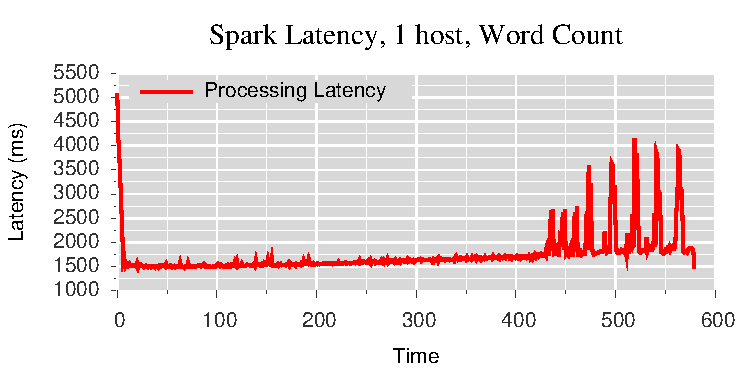
\includegraphics[width=1\linewidth]{figures/sp1_latency.pdf}
%\vspace{-0.3in}
\caption{Average latency to process tuples for a single Spark host. Similar to Figure~\ref{sb1-tput} we sent 1KB tuples at a slowly ramped up rate from 1K tuples/sec to 30k tuples/sec with a step size of 500 tuples/sec. The sending rate remained constant for 10 seconds before transitioning to the next throughput. The astute reader will notice that the latency spike in this graph occurs at the same time as the loss in throughput consistency in Figure~\ref{sb1-tput}}
\label{fig:label-me-if-you-want}
\end{figure}



\section{Acknowledgments}
Thank you.

%
% The following two commands are all you need in the
% initial runs of your .tex file to
% produce the bibliography for the citations in your paper.
\bibliographystyle{abbrv}
\bibliography{bibdata}  % sigproc.bib is the name of the Bibliography in this case
% You must have a proper ".bib" file
%  and remember to run:
% latex bibtex latex latex
% to resolve all references
%
% ACM needs 'a single self-contained file'!
%
%APPENDICES are optional
%\balancecolumns
%\appendix
%Appendix A

\balancecolumns
% That's all folks!
\end{document}
